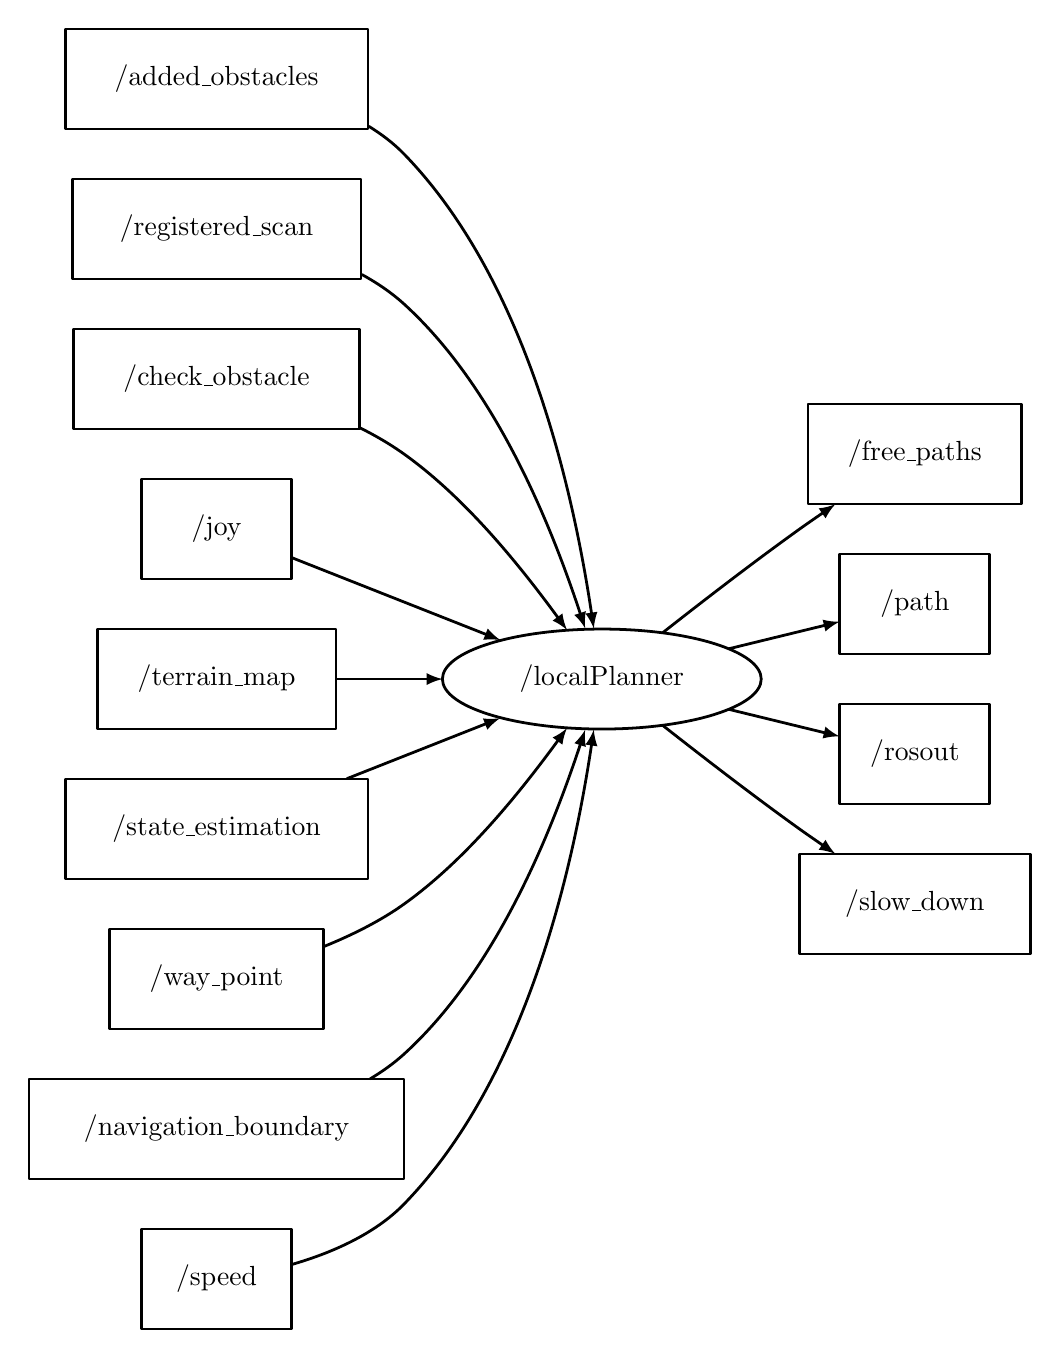
\begin{tikzpicture}[>=latex,line join=bevel,]
  \pgfsetlinewidth{1bp}
%%
\pgfsetcolor{black}
  % Edge: t___added_obstacles -> n___localPlanner
  \draw [->] (122.25bp,433.02bp) .. controls (126.91bp,430.16bp) and (131.27bp,426.85bp)  .. (135.0bp,423.0bp) .. controls (178.86bp,377.8bp) and (195.74bp,302.78bp)  .. (203.31bp,252.17bp);
  % Edge: n___localPlanner -> t___free_paths
  \draw [->] (228.11bp,250.68bp) .. controls (241.92bp,261.55bp) and (260.52bp,275.91bp)  .. (277.39bp,288.0bp) .. controls (278.81bp,289.02bp) and (280.26bp,290.04bp)  .. (290.27bp,296.95bp);
  % Edge: n___localPlanner -> t___path
  \draw [->] (251.9bp,244.9bp) .. controls (261.86bp,247.33bp) and (272.29bp,249.88bp)  .. (291.82bp,254.64bp);
  % Edge: n___localPlanner -> t___rosout
  \draw [->] (251.9bp,223.1bp) .. controls (261.86bp,220.67bp) and (272.29bp,218.12bp)  .. (291.82bp,213.36bp);
  % Edge: n___localPlanner -> t___slow_down
  \draw [->] (228.11bp,217.32bp) .. controls (241.92bp,206.45bp) and (260.52bp,192.09bp)  .. (277.39bp,180.0bp) .. controls (278.81bp,178.98bp) and (280.26bp,177.96bp)  .. (290.27bp,171.05bp);
  % Edge: t___registered_scan -> n___localPlanner
  \draw [->] (119.77bp,379.65bp) .. controls (125.26bp,376.64bp) and (130.48bp,373.11bp)  .. (135.0bp,369.0bp) .. controls (167.15bp,339.73bp) and (186.98bp,292.29bp)  .. (200.19bp,252.26bp);
  % Edge: t___check_obstacle -> n___localPlanner
  \draw [->] (119.23bp,324.39bp) .. controls (124.76bp,321.61bp) and (130.14bp,318.48bp)  .. (135.0bp,315.0bp) .. controls (155.87bp,300.06bp) and (174.64bp,277.7bp)  .. (193.67bp,251.65bp);
  % Edge: t___joy -> n___localPlanner
  \draw [->] (94.533bp,277.72bp) .. controls (113.09bp,270.39bp) and (138.51bp,260.34bp)  .. (169.71bp,248.02bp);
  % Edge: t___terrain_map -> n___localPlanner
  \draw [->] (110.63bp,234.0bp) .. controls (119.5bp,234.0bp) and (129.07bp,234.0bp)  .. (148.87bp,234.0bp);
  % Edge: t___state_estimation -> n___localPlanner
  \draw [->] (114.4bp,198.13bp) .. controls (129.16bp,203.96bp) and (145.49bp,210.41bp)  .. (169.58bp,219.93bp);
  % Edge: t___way_point -> n___localPlanner
  \draw [->] (106.35bp,137.8bp) .. controls (116.16bp,141.79bp) and (126.39bp,146.84bp)  .. (135.0bp,153.0bp) .. controls (155.87bp,167.94bp) and (174.64bp,190.3bp)  .. (193.67bp,216.35bp);
  % Edge: t___navigation_boundary -> n___localPlanner
  \draw [->] (122.77bp,90.063bp) .. controls (127.16bp,92.679bp) and (131.31bp,95.645bp)  .. (135.0bp,99.0bp) .. controls (167.15bp,128.27bp) and (186.98bp,175.71bp)  .. (200.19bp,215.74bp);
  % Edge: t___speed -> n___localPlanner
  \draw [->] (94.726bp,23.288bp) .. controls (108.3bp,27.23bp) and (124.24bp,33.912bp)  .. (135.0bp,45.0bp) .. controls (178.86bp,90.196bp) and (195.74bp,165.22bp)  .. (203.31bp,215.83bp);
  % Node: t___added_obstacles
\begin{scope}
  \definecolor{strokecol}{rgb}{0.0,0.0,0.0};
  \pgfsetstrokecolor{strokecol}
  \draw (122.0bp,468.0bp) -- (13.0bp,468.0bp) -- (13.0bp,432.0bp) -- (122.0bp,432.0bp) -- cycle;
  \draw (67.5bp,450.0bp) node {/added\_obstacles};
\end{scope}
  % Node: n___localPlanner
\begin{scope}
  \definecolor{strokecol}{rgb}{0.0,0.0,0.0};
  \pgfsetstrokecolor{strokecol}
  \draw (206.19bp,234.0bp) ellipse (57.39bp and 18.0bp);
  \draw (206.19bp,234.0bp) node {/localPlanner};
\end{scope}
  % Node: t___free_paths
\begin{scope}
  \definecolor{strokecol}{rgb}{0.0,0.0,0.0};
  \pgfsetstrokecolor{strokecol}
  \draw (357.39bp,333.0bp) -- (280.39bp,333.0bp) -- (280.39bp,297.0bp) -- (357.39bp,297.0bp) -- cycle;
  \draw (318.89bp,315.0bp) node {/free\_paths};
\end{scope}
  % Node: t___path
\begin{scope}
  \definecolor{strokecol}{rgb}{0.0,0.0,0.0};
  \pgfsetstrokecolor{strokecol}
  \draw (345.89bp,279.0bp) -- (291.89bp,279.0bp) -- (291.89bp,243.0bp) -- (345.89bp,243.0bp) -- cycle;
  \draw (318.89bp,261.0bp) node {/path};
\end{scope}
  % Node: t___rosout
\begin{scope}
  \definecolor{strokecol}{rgb}{0.0,0.0,0.0};
  \pgfsetstrokecolor{strokecol}
  \draw (345.89bp,225.0bp) -- (291.89bp,225.0bp) -- (291.89bp,189.0bp) -- (345.89bp,189.0bp) -- cycle;
  \draw (318.89bp,207.0bp) node {/rosout};
\end{scope}
  % Node: t___slow_down
\begin{scope}
  \definecolor{strokecol}{rgb}{0.0,0.0,0.0};
  \pgfsetstrokecolor{strokecol}
  \draw (360.39bp,171.0bp) -- (277.39bp,171.0bp) -- (277.39bp,135.0bp) -- (360.39bp,135.0bp) -- cycle;
  \draw (318.89bp,153.0bp) node {/slow\_down};
\end{scope}
  % Node: t___registered_scan
\begin{scope}
  \definecolor{strokecol}{rgb}{0.0,0.0,0.0};
  \pgfsetstrokecolor{strokecol}
  \draw (119.5bp,414.0bp) -- (15.5bp,414.0bp) -- (15.5bp,378.0bp) -- (119.5bp,378.0bp) -- cycle;
  \draw (67.5bp,396.0bp) node {/registered\_scan};
\end{scope}
  % Node: t___check_obstacle
\begin{scope}
  \definecolor{strokecol}{rgb}{0.0,0.0,0.0};
  \pgfsetstrokecolor{strokecol}
  \draw (119.0bp,360.0bp) -- (16.0bp,360.0bp) -- (16.0bp,324.0bp) -- (119.0bp,324.0bp) -- cycle;
  \draw (67.5bp,342.0bp) node {/check\_obstacle};
\end{scope}
  % Node: t___joy
\begin{scope}
  \definecolor{strokecol}{rgb}{0.0,0.0,0.0};
  \pgfsetstrokecolor{strokecol}
  \draw (94.5bp,306.0bp) -- (40.5bp,306.0bp) -- (40.5bp,270.0bp) -- (94.5bp,270.0bp) -- cycle;
  \draw (67.5bp,288.0bp) node {/joy};
\end{scope}
  % Node: t___terrain_map
\begin{scope}
  \definecolor{strokecol}{rgb}{0.0,0.0,0.0};
  \pgfsetstrokecolor{strokecol}
  \draw (110.5bp,252.0bp) -- (24.5bp,252.0bp) -- (24.5bp,216.0bp) -- (110.5bp,216.0bp) -- cycle;
  \draw (67.5bp,234.0bp) node {/terrain\_map};
\end{scope}
  % Node: t___state_estimation
\begin{scope}
  \definecolor{strokecol}{rgb}{0.0,0.0,0.0};
  \pgfsetstrokecolor{strokecol}
  \draw (122.0bp,198.0bp) -- (13.0bp,198.0bp) -- (13.0bp,162.0bp) -- (122.0bp,162.0bp) -- cycle;
  \draw (67.5bp,180.0bp) node {/state\_estimation};
\end{scope}
  % Node: t___way_point
\begin{scope}
  \definecolor{strokecol}{rgb}{0.0,0.0,0.0};
  \pgfsetstrokecolor{strokecol}
  \draw (106.0bp,144.0bp) -- (29.0bp,144.0bp) -- (29.0bp,108.0bp) -- (106.0bp,108.0bp) -- cycle;
  \draw (67.5bp,126.0bp) node {/way\_point};
\end{scope}
  % Node: t___navigation_boundary
\begin{scope}
  \definecolor{strokecol}{rgb}{0.0,0.0,0.0};
  \pgfsetstrokecolor{strokecol}
  \draw (135.0bp,90.0bp) -- (0.0bp,90.0bp) -- (0.0bp,54.0bp) -- (135.0bp,54.0bp) -- cycle;
  \draw (67.5bp,72.0bp) node {/navigation\_boundary};
\end{scope}
  % Node: t___speed
\begin{scope}
  \definecolor{strokecol}{rgb}{0.0,0.0,0.0};
  \pgfsetstrokecolor{strokecol}
  \draw (94.5bp,36.0bp) -- (40.5bp,36.0bp) -- (40.5bp,0.0bp) -- (94.5bp,0.0bp) -- cycle;
  \draw (67.5bp,18.0bp) node {/speed};
\end{scope}
%
\end{tikzpicture}
